\documentclass[11pt, leqno]{scrartcl}
\usepackage{polski}
\usepackage[polish]{babel}

\usepackage{graphicx, float, caption, subcaption}
\usepackage{tabularx, multirow, hyperref, enumitem}
\usepackage{listings, xcolor}
\usepackage{amsmath, amssymb}
%\usepackage{minted}

\hypersetup{
    colorlinks=true,
    linkcolor=black,
    urlcolor=black,
    citecolor=black
}

\definecolor{md-black}{rgb}{0.12, 0.12, 0.12}
\definecolor{md-teal}{rgb}{0.38, 0.79, 0.69}
\definecolor{md-mauve}{rgb}{0.76, 0.52, 0.75}
\definecolor{md-yellow}{rgb}{0.86, 0.86, 0.67}
\definecolor{md-green}{rgb}{0.13, 0.55, 0.13}
\definecolor{md-red}{rgb}{0.82, 0.10, 0.14}
\definecolor{md-purple}{rgb}{0.69, 0.33, 0.73}
\definecolor{md-orange}{rgb}{0.96, 0.42, 0.18}
\definecolor{md-gray}{rgb}{0.44, 0.46, 0.51}
\lstset{
    language=Python,
    basicstyle=\color{md-teal}\ttfamily,
    keywordstyle=\color{md-mauve},
    commentstyle=\color{md-green},
    stringstyle=\color{md-red},
    numbers=left,
    numberstyle=\small\color{md-gray}\ttfamily,
    stepnumber=1,
    numbersep=5pt,
    backgroundcolor=\color{md-black},
    showspaces=false,
    showstringspaces=false,
    showtabs=false,
    frame=none,
    tabsize=4,
    captionpos=b,
    breaklines=true,
    breakatwhitespace=false,
    escapeinside={\%*}{*)},
    numbersep=-10pt,
    morekeywords={as},
    classoffset=1,
    morekeywords={quad, quad_vec, trapz, simps, linregress,
        newton},
    keywordstyle=\color{md-yellow},
    classoffset=0
}

\graphicspath{{../images/}}

\title{Laboratorium 9 - Równania różniczkowe zwyczajne}
\author{Mateusz Podmokły - II rok Informatyka WI}
\date{16 maj 2024}

\begin{document}
    \maketitle
    \section{Treść zadania}
    \textbf{Zadanie 1.} Przedstaw każde z poniższych równań
    różniczkowych zwyczajnych jako równoważny układ równań
    pierwszego rzędu (ang. first-order system of ODEs):
    \begin{enumerate}
        \item równanie Van der Pol'a:
            \[
                y''=y'(1-y^2)-y
            \]
        \item równanie Blasiusa:
            \[
                y'''=-yy''
            \]
        \item II zasada dynamiki Newtona dla problemu dwóch
            ciał:
            \[
                y_1''=-\frac{GMy_1}{(y_1^2+y_2^2)^{\frac{3}{2}}}
            \]
            \[
                y_2''=-\frac{GMy_2}{(y_1^2+y_2^2)^{\frac{3}{2}}}
            \]
    \end{enumerate}

    \subsection*{}
    \textbf{Zadanie 2.} Dane jest równanie różniczkowe
    zwyczajne
    \[
        y'=-5y
    \]
    z warunkiem początkowym $y(0) = 1$. Równanie rozwiązujemy
    numerycznie z krokiem $h = 0.5$.
    \begin{enumerate}
        \item Analityczna stabilność. Wyjaśnij, czy rozwiązania
            powyższego równania są stabilne?
        \item Numeryczna stabilność. Wyjaśnij, czy metoda
            Euler'a jest stabilna dla tego równania z użytym
            krokiem $h$?
        \item Oblicz numerycznie wartości przybliżonego
            rozwiązania dla $t = 0.5$ metodą Euler'a.
        \item Wyjaśnij, czy niejawna metoda Euler'a jest
            stabilna dla tego równania z użytym krokiem $h$?
        \item Oblicz numerycznie wartości przybliżonego
            rozwiązania dla $t = 0.5$ niejawną metodą Euler'a.
    \end{enumerate}

    \subsection*{}
    \textbf{Zadanie 3.} Model Kermack'a-McKendrick'a przebiegu
    epidemii w populacji opisany jest układem równań
    różniczkowych:
    \begin{align*}
        &S'=-\frac{\beta}{N}IS \\
        &I'=\frac{\beta}{N}IS-\gamma I \\
        &R'=\gamma I
    \end{align*}
    gdzie \\
    S - liczba osób zdrowych, podatnych na zainfekowanie \\
    I - liczba osób zainfekowanych i roznoszących infekcję \\
    R - liczba osób ozdrowiałych

    \subsubsection*{}
    Liczba N to liczba osób w populacji. Parametr $\beta$
    reprezentuje współczynnik zakaźności. Parametr $\gamma$
    reprezentuje współczynnik wyzdrowień. Wartość
    $\frac{1}{\gamma}$ reprezentuje średni czas choroby. \\
    Założenia modelu:
    \begin{itemize}
        \item przyrost liczby osób zakażonych jest proporcjonalny
            do liczby osób zakażonych oraz do liczby osób
            podatnych,
        \item przyrost liczby osób odpornych lub zmarłych jest
            wprost proporcjonalny do liczby aktualnie chorych,
        \item okres inkubacji choroby jest zaniedbywalnie krótki,
        \item populacja jest wymieszana.
    \end{itemize}
    Jako wartości początkowe ustal:
    \[
        S(0)=762
    \]
    \[
        I(0)=1
    \]
    \[
        R(0)=0
    \]
    Przyjmij też $N=S(0)+I(0)+R(0)=763$ oraz $\beta =1$.
    Zakładając, że średni czas trwania grypy wynosi
    $\frac{1}{\gamma}=7$ dni, przyjmij $\gamma =\frac{1}{7}$. \\
    Całkując od $t=0$ do $t=14$ z krokiem 0.2, rozwiąż powyższy
    układ równań:
    \begin{itemize}
        \item jawną metodą Euler'a
            \[
                y_{k+1}=y_k+h_kf(t_k, y_k)
            \]
        \item niejawną metodą Euler'a
            \[
                y_{k+1}=y_k+h_kf(t_{k+1}, y_{k+1})
            \]
        \item metodą Rungego-Kutty czwartego rzędu (RK4)
            \[
                y_{k+1}=y_k+\frac{h_k}{6}(k_1+2k_2+2k_3+k_4)
            \]
            \begin{align*}
                &k_1=f(t_k,y_k) \\
                &k_2=f \left( t_k+\frac{h_k}{2},
                    y_k+\frac{h_kk_1}{2} \right) \\
                &k_3=f \left( t_k+\frac{h_k}{2},
                    y_k+\frac{h_kk_2}{2} \right) \\
                &k_4=f(t_k+h_k,y_k+h_kk_3)
            \end{align*}
    \end{itemize}
    Wykonaj następujące wykresy:
    \begin{itemize}
        \item Dla każdej metody przedstaw na wspólnym rysunku
            wykresy komponentów rozwiązania ($S$, $I$, $R$) jako
            funkcje $t$ (3 wykresy).
        \item Na wspólnym rysunku przedstaw wykresy funkcji
            $S(t)+I(t)+R(t)$ znalezione przez każdą metodę
            (1 wykres). Czy niezmiennik $S(t)+I(t)+R(t) \equiv N$
            jest zachowany?
    \end{itemize}

    \section{Specyfikacja użytego środowiska}
    Specyfikacja:
    \begin{itemize}
        \item Środowisko: Visual Studio Code,
        \item Język programowania: Python,
        \item System operacyjny: Microsoft Windows 11,
        \item Architektura systemu: x64.
    \end{itemize}

    \section{Rozwiązanie problemu}
    \subsection{Biblioteki}
    W realizacji rozwiązania wykorzystane zostały następujące
    biblioteki:
    \begin{lstlisting}
    import numpy as np
    import matplotlib.pyplot as plt
    \end{lstlisting}

    \subsection{Zadanie 1.}
    Każde równanie w postaci równania różniczkowego zwyczajnego
    zostanie przekształcone równoważnie do układu równań
    pierwszego rzędu.

    \subsubsection{Równanie 1.}
    Mamy równanie
    \[
        y''=y'(1-y^2)-y
    \]
    Zastosujemy podstawienie
    \[
        z=y'
    \]
    Otrzymuejmy równoważny układ równań
    \[
        \begin{cases}
            y'=z \\
            z'=z(1-y^2)-y
        \end{cases}
    \]

    \subsubsection{Równanie 2.}
    Mamy równanie
    \[
        y'''=-yy''
    \]
    Stosujemy analogiczne podstawienia
    \[
        z=y'
    \]
    \[
        w=z'
    \]
    Otrzymuejmy układ równań
    \[
        \begin{cases}
            y'=z \\
            z'=w \\
            w'=-yw
        \end{cases}
    \]

    \subsubsection{Równanie 3.}
    Mamy równanie
    \[
        y_1''=-\frac{GMy_1}{(y_1^2+y_2^2)^{\frac{3}{2}}}
    \]
    \[
        y_2''=-\frac{GMy_2}{(y_1^2+y_2^2)^{\frac{3}{2}}}
    \]
    Stosujemy analogiczne podstawienia
    \[
        z_1=y_1'
    \]
    \[
        z_2=y_2'
    \]
    Otrzymuejmy układ równań
    \[
        \begin{cases}
            y_1'=z_1 \\
            y_2'=z_2 \\
            z_1'=-\frac{GMy_1}{(y_1^2+y_2^2)^{\frac{3}{2}}} \\
            z_2'=-\frac{GMy_2}{(y_1^2+y_2^2)^{\frac{3}{2}}}
        \end{cases}
    \]

    \subsection{Zadanie 2.}
    \subsubsection{Analityczna stabilność}
    Mamy równanie
    \[
        y'=-5y
    \]
    z warunkiem początkowym
    \[
        y(0)=1
    \]
    Możemy je rozwiązać analitycznie w prosty sposób metodą
    separacji zmiennych. Otrzymujemy rozwiązanie
    \[
        y(t)=y_0e^{-5t}
    \]
    gdzie
    \[
        y_0=y(0)=1
    \]
    Teraz sprawdźmy stabilność otrzymanego rozwiązania.
    Równanie różniczkowe jest stabilne, jeśli dla każdego
    $\epsilon > 0$ istnieje $\delta > 0$ takie, że jeśli
    początkowe odchylenie
    \[
        |y(0)-y_0|<\delta
    \]
    to
    \[
        |y(t)-\hat{y}(t)|<\epsilon
    \]
    dla każdego $t \geq 0$. \\ 
    Rozważmy zaburzenie początkowego warunku
    \[
        y(0)=y_0
    \]
    Niech
    \[
        \hat{y}(0)=y_0+\delta
    \]
    Mamy wtedy rozwiązanie równania dla początkowego warunku
    \[
        \hat{y}(t)=(y_0+\delta)e^{-5t}
    \]
    Możemy podstawić
    \[
        |y(t)-\hat{y}(t)|=|y_0e^{-5t}-(y_0+\delta)e^{-5t}|=
            |\delta e^{-5t}|
    \]
    Wiadomo, że $e^{-5t} \leq 1$ dla każdego $t \geq 0$, więc
    \[
        |\delta e^{-5t}| \leq |\delta|
    \]
    Możemy wtedy wybrać $\delta$ takie, że
    $|\delta | \leq \epsilon $. Wtedy
    \[
        |y(t)-\hat{y}(t)| < \epsilon
    \]
    Oznacza to, że rozwiązania tego równania są stabilne.

    \subsubsection{Numeryczna stabilność}
    Dla równań różniczkowych postaci
    \[
        y'=\lambda y
    \]
    gdzie $\lambda \in \mathbb{R}$, warunek stabilności
    numerycznej metody Euler'a dany jest wzorem
    \[
        |1+h\lambda|<1
    \]
    Mamy $\lambda =-5$, więc po przekształceniu równoważnym
    podanego warunku otrzymujemy
    \[
        0<h<0.4
    \]
    Z tego wynika, że dla tego równania z krokiem $h=0.5$
    metoda Euler'a nie jest stabilna numerycznie.

    \subsubsection{Metoda Euler'a}
    Rozwiązanie równania postaci
    \[
        y'=f(y,t)
    \]
    o warunku początkowym $y(t_0)=y_0$ i kroku $h$, z punktami
    $t_i$ na osi OX:
    \[
        t_{n+1}=t_n+h,\quad n=0,1,2,\dots
    \]
    za pomocą metody Euler'a możemy otrzymać ze wzoru:
    \[
        y_{n+1}=y_n+hf(y_n,t_n)
    \]
    
    \subsubsection{Stabilność niejawnej metody Euler'a}
    Dla równań różniczkowych postaci
    \[
        y'=\lambda y
    \]
    gdzie $\lambda \in \mathbb{R}$, warunek stabilności
    numerycznej niejawnej metody Euler'a dany jest wzorem
    \[
        \left| \frac{1}{1-h\lambda} \right| <1
    \]
    Mamy $\lambda =-5$, więc po przekształceniu równoważnym
    podanego warunku otrzymujemy
    \[
        h>0
    \]
    Z tego wynika, że dla dowolnego kroku $h>0$ niejawna metoda
    Euler'a jest stabilna numerycznie.

    \subsubsection{Niejawna metoda Euler'a}
    Rozwiązanie równania postaci
    \[
        y'=f(y,t)
    \]
    o warunku początkowym $y(t_0)=y_0$ i kroku $h$, z punktami
    $t_i$ na osi OX:
    \[
        t_{n+1}=t_n+h,\quad n=0,1,2,\dots
    \]
    za pomocą niejawnej metody Euler'a możemy otrzymać ze
    wzoru:
    \[
        y_{n+1}=y_n+hf(y_{n+1},t_{n+1})
    \]
    Mamy równanie
    \[
        y'=-5y
    \]
    o warunku początkowym $y(0)=1$ i kroku $h=0.5$.
    Podstawiamy $f(y,t)$ do wzoru
    \[
        y_{n+1}=y_n+h(-5y_{n+1})
    \]
    Przekształcając równoważnie otrzymujemy wzór na $y_{n+1}$
    \[
        y_{n+1}=\frac{y_n}{5h+1}
    \]

    \subsection{Zadanie 3.}
    \subsubsection{Jawna metoda Euler'a}
    Układ równań postaci
    \[
        y_1'=f_1(y_1,y_2,y_3,t)
    \]
    \[
        y_2'=f_2(y_1,y_2,y_3,t)
    \]
    \[
        y_3'=f_3(y_1,y_2,y_3,t)
    \]
    rozwiązujemy korzystając ze wzoru
    \[
        y_{n+1}=y_n+hf(y_n,t_n)
    \]
    \subsubsection{Niejawna metoda Euler'a}
    Układ równań postaci
    \[
        y_1'=f_1(y_1,y_2,y_3,t)
    \]
    \[
        y_2'=f_2(y_1,y_2,y_3,t)
    \]
    \[
        y_3'=f_3(y_1,y_2,y_3,t)
    \]
    rozwiązujemy korzystając ze wzoru
    \[
        y_{n+1}=y_n+hf(y_{n+1}, t_{n+1})
    \]
    Podstawiamy układ równań do wzoru
    \[
        \begin{cases}
            S_{n+1}=S_n-h\frac{\beta}{N}I_{n+1}S_{n+1} \\
            I_{n+1}=I_n+h \left( \frac{\beta}{N}I_{n+1}S_{n+1}
                -\gamma I_{n+1} \right) \\
            R_{n+1}=R_n+h\gamma I_{n+1}
        \end{cases}
    \]
    Do rozwiązania układu równań wykorzystałem funkcję z biblioteki
    \texttt{SciPy}
    \[
        \texttt{scipy.optimize.fsolve}
    \]
    \subsubsection{Metoda Rungego-Kutty czwartego rzędu (RK4)}
    Układ równań postaci
    \[
        y_1'=f_1(y_1,y_2,y_3,t)
    \]
    \[
        y_2'=f_2(y_1,y_2,y_3,t)
    \]
    \[
        y_3'=f_3(y_1,y_2,y_3,t)
    \]
    rozwiązujemy korzystając ze wzoru
    \[
        y_{n+1}=y_n+\frac{h}{6}(k_1+2k_2+2k_3+k_4)
    \]
    \begin{align*}
        &k_1=f(y_n,t_n) \\
        &k_2=f \left( t_n+\frac{h}{2},
            y_n+\frac{hk_1}{2} \right) \\
        &k_3=f \left( t_n+\frac{h}{2},
            y_n+\frac{hk_2}{2} \right) \\
        &k_4=f(t_n+h,y_n+hk_3)
    \end{align*}

    \subsubsection{Szacowanie współczynników}
    Oszacowanie wartości współczynników wykonałem z użyciem
    jawnej metody Euler'a danej wzorem
    \[
        y_{n+1}=y_n+hf(y_n,t_n)
    \]
    Do minimalizacji funkcji kosztu metodą Neldera-Meada użyłem
    funkcji z biblioteki \texttt{SciPy}
    \[
        \texttt{scipy.optimize.minimize}
    \]
    
    \section{Przedstawienie wyników}
    \subsection{Zadanie 2.}
    \subsubsection{Jawna metoda Euler'a}
    Dla równania
    \[
        y'=-5y
    \]
    oraz $y(0)=1$ i $h=0.5$ otrzymujemy wynik
    \[
        y(0.5)=-1.5
    \]
    a więc różni się on znacznie od tego wyznaczonego
    analitycznie, który wynosi
    \[
        y_{true}(0.5) \approx 0.082
    \]
    Rozbieżność wynika prawdopodobnie z braku stabilności
    numerycznej tej metody z przyjętym krokiem $h$. Dla
    $h=0.1$ wynik to już
    \[
        y(0.5) \approx 0.031
    \]

    \subsubsection{Niejawna metoda Euler'a}
    Po wykonaniu obliczeń z wykorzystaniem wyprowadzonego
    wzoru otrzymujemy wynik
    \[
        y(0.5) \approx 0.286
    \]
    Jest on znacznie lepszy niż w przypadku jawnej
    metody Euler'a dla kroku $h=0.5$. Zmieńmy krok
    na $h=0.1$. Otrzymujemy wtedy wynik
    \[
        h(0.5) \approx 0.132
    \]
    \subsection{Zadanie 3.}
    \subsubsection{Wykresy przebiegu epidemii}
    \begin{figure}[H]
        \centering
        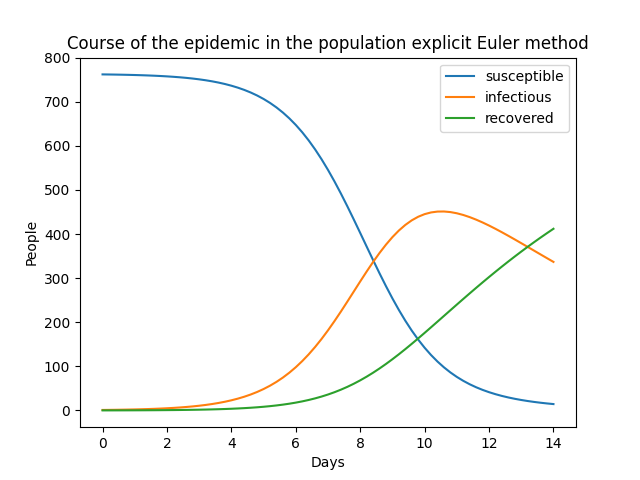
\includegraphics[width=0.7\linewidth]{explicit_euler.png}
        \caption{Przebieg epidemii w populacji otrzymany
            jako rozwiązanie układu równań różniczkowych jawną
            metodą Euler'a.}
    \end{figure}
    \begin{figure}[H]
        \centering
        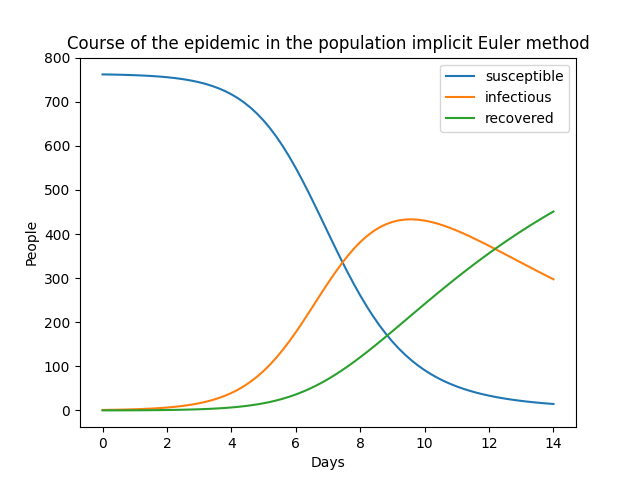
\includegraphics[width=0.7\linewidth]{implicit_euler.png}
        \caption{Przebieg epidemii w populacji otrzymany
            jako rozwiązanie układu równań różniczkowych niejawną
            metodą Euler'a.}
    \end{figure}
    \begin{figure}[H]
        \centering
        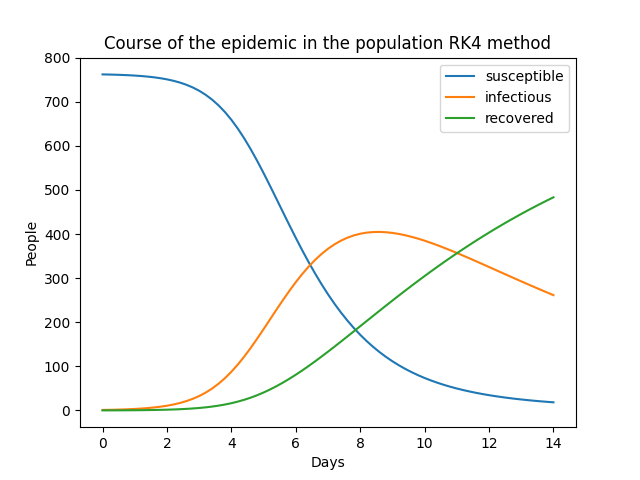
\includegraphics[width=0.7\linewidth]{RK4.png}
        \caption{Przebieg epidemii w populacji otrzymany
            jako rozwiązanie układu równań różniczkowych metodą
            Rungego-Kutty rzędu czwartego (RK4).}
    \end{figure}
    \begin{figure}[H]
        \centering
        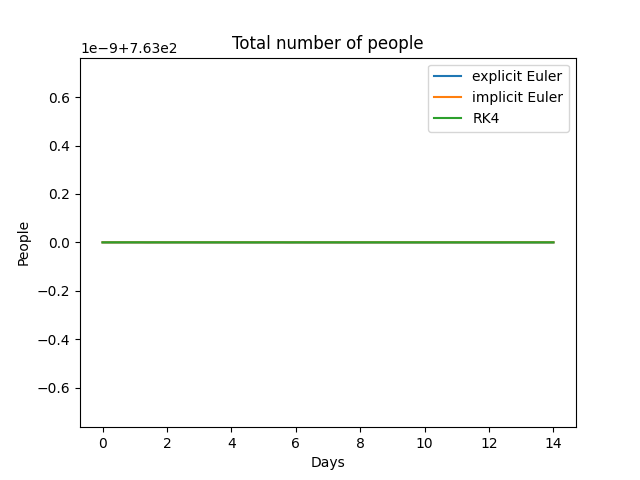
\includegraphics[width=0.7\linewidth]{total_people.png}
        \caption{Łączna wielkość populacji w czasie.}
    \end{figure}

    \subsubsection{Szacowanie współczynników}
    Dla funkcji kosztu
    \[
        L(\theta)=\sum_{i=0}^{T}(I_i-\hat{I_i})^2
    \]
    otrzymane wartości współczynników to:
    \[
        \beta \approx 2.31
    \]
    \[
        \gamma \approx 0.3
    \]
    \[
        R_0=\frac{\beta}{\gamma} \approx 7.81
    \]
    a dla funkcji
    \[
        L(\theta)=-\sum_{i=0}^{T}I_iln\hat{I_i}+
            \sum_{i=0}^{T}\hat{I_i}
    \]
    współczynniki wynoszą
    \[
        \beta \approx 2.34
    \]
    \[
        \gamma \approx 0.31
    \]
    \[
        R_0=\frac{\beta}{\gamma} \approx 7.63
    \]

    \section{Wnioski}
    Niejawna metoda Euler'a okazała się bardziej stabilna niż
    jawna metoda Euler'a, ale charakteryzuje się mniejszą
    dokładnością zwracanych wyników. Zarówno metoda Euler'a,
    jak i metoda Rungego-Kutty czwartego rzędu (RK4), są
    skutecznymi narzędziami do rozwiązywania układów równań
    różniczkowych. Należy jednak pamiętać o odpowiednim doborze
    kroku $h$ w celu zachowania stabilności metody.

    \section{Bibliografia}
    \url{https://pl.wikipedia.org/wiki/Metoda_Eulera} \\
    \url{https://pl.wikipedia.org/wiki/Algorytm_Rungego-Kutty} \\
    \url{https://pl.wikipedia.org/wiki/Metody_Lapunowa} \\
    \url{https://pl.wikipedia.org/wiki/Metoda_Neldera-Meada}
    
\end{document}
